\section{Computational Pipeline}

\subsection{R-K Toolkit}

 To build the RK-Diagrams and RK-Models, we implemented a generalizable package called RK-Toolkit \cite{rktoolkit}. The R-K toolkit is a framework to build a component called an RK-Pipeline (described in section 4.4), and can be found open sourced, at \url{https://github.com/andorsk/rk_toolkit}. The RK-Toolkit was built in python, and converts the core mathematical concepts described in this paper into computational representations that can be used on real data. Similar to how other libraries such as Sci-Kit \cite{a2021_scikitlearn} provide base components like the Pipeline object \cite{a2021_61}, to be extended later by a user or by native extensions, RK-Toolkit operates similarly by providing the base building blocks such as a R-K Pipeline and R-K Diagram, to be extended by the user or by native representations. As an example, if one were to want to classify a Hodgkins vs. Non-Hodgkins disease along with their 4 stages of metastasis as distinct topological signatures that are divergent from healthy patients, one could construct their own R-K Pipeline out of the toolkit, to potentially generate unique topological structures and R-K Diagrams. The R-K Toolkit's design was done explicitly with the intent to be extended later, with the expectations that new and more robust methods will be included into framework over time.Any computation carried out using the R-K Toolkit leading to a set of actions to build and generate R-K diagrams can be defined as the \textbf{\textit{R-K Workflow}}.

The R-K Toolkit provides many advantages over starting from scratch. We submit that there are 9 main advantages to using the R-K Toolkit for building future models.

\begin{enumerate}
    \item{The R-K Toolkit provides in build validation for components, such as adherence to a DAG and valid transforms}
    \item{A pipeline framework is provided to chain steps together with accordance to the computational steps to be described below}
    \item{Visualization's are provided to assist with rendering of RK-Models and converting them into RK-Diagrams.}
    \item{Pre-built transforms provide baseline transforms for testing }
    \item{Various Optimizations and Machine Learning implementations will be present in the RK-Toolkit for various use cases}
    \item{Built in mechanisms to provide inverse operations}
    \item{Our toolkit allows for plug and play of well defined domain ontologies pertaining to knowledge graph or custom ontologies pertaining to a structured dataset}
    \item{This framework can be extended to include many datasets as long as it conforms to the data requirements}
    \item{The R-K Pipeline is built in such a way that it could in theory support streams for real time classification and identification use cases, however future work would be required to update this feature in further details.}
\end{enumerate}

To apply the toolkit to a dataset, one would import the relevant components into their code (similar to how you would Sci-Kit), define a RK-Pipeline, and then run the pipeline. It is entirely in the control of the user \textit{how} they desire to build their pipeline as most pipelines will vary across domains and data. The intent with this paper, and with the core concepts of the R-K Pipelines, are that despite the divergence of implementations, the foundational building blocks of an R-K Pipeline will always remain the same.

We acknowledge that this is the first implementation of the R-K toolkit, but it has shown good promise with useful results on the below use cases, but future work is required to make it more robust for it's application across different domains.

\subsubsection{R-K WorkBench}

To help users get started quicker, we provide a docker image called RK-Workbench \cite{andorsk_2021_andorskrkworkbench}, which wraps the ML-Workspace \cite{mltooling_2021_mltoolingmlworkspace} with packages relevant to building RK-Diagrams built into the core image. The README file details how to use it for the purpose of independent use by researchers and programmers. 

\subsection{Data Qualification Criterion}

Let us now address the data qualification criteria and its associated constraints for the R-K pipeline that would allow for the accurate execution of our analytical framework pertaining to "Event-Driven" Topological Graph Analysis. In this approach, we shall not be addressing the study of unstructured point-cloud data as addressed in the traditional TDA frameworks of the past \cite{01.9_2007MapperPBG} \cite{02_carlsson2009topology} \cite{02.3_2017introductionTDA} but focus on a subset of data with well-defined hierarchical features that can be extracted automatically as a part of this pipeline and linked to the corresponding interdependencies of columns and rows in relation to the chosen context for the purpose of segregation (ref:4.5.5) and classification of meaningful events and entities within such datasets.

We start by defining $D_i (\forall i \in N)$ as the input dataset to the R-K Toolkit; where $M_j (\forall j \in N)$ is a measure within the dataset. For example, Mass and Spin are measures on the LIGO dataset.\cite{00_LIGOOpenSciData}Then for any such dataset $D_i$ containing $M_j$ measures to be accepted into the R-K Model Framework, it must adhere to the following constraints:

\begin{itemize}
	\item It must be able to derive a hierarchy of relationships between measures such that the Dendogram of hierarchy $H$ describes how one measure relates to another.
	\item It must be able to segregate independent variables and their corresponding dependencies in separate attribute clusters of the "Event-Node".
	\item It must have at least 3 mutually-independent variables pertaining to the well-defined attributes of "Physical Systems" \&  "Non-Physical Systems" as detailed below.
\end{itemize}

\subsubsection{Physical Systems}
\label{sec:PhysicalSystems}

The Datasets pertaining to “Physical Systems” must contain at least \textit{3 mutually independent variables} related to the 7 Fundamental Quantities of Physics \cite{23.0_DimensionalAnalysis} to meet the the minimum criteria for generating an  R-K Diagram in accordance with consistent Topological Properties that can be distinguished using appropriate filtering \& divergence criteria.

In physics, a physical system is a portion of the physical universe chosen for analysis. Everything outside the system is known as the environment. The environment is ignored except for its effects on the system. Any system defined in the realm of science and engineering can be referred to as a physical system with independent variables that have the following fundamental dimensions: \textit{mass, length, time, temperature, electricity, luminous intensity \& count/amount of substance/matter}. \cite{23.1_7FundamentalQuants} An example of hierarchical clustering using the well defined relationships of dependent and independent variables pertaining to physical systems is shown below with respect to a fundamental structural graph in the R-K model framework, which can be filtered specifically to obtain unique event-driven R-K Diagrams. 

\begin{figure}[H]
	\centering
	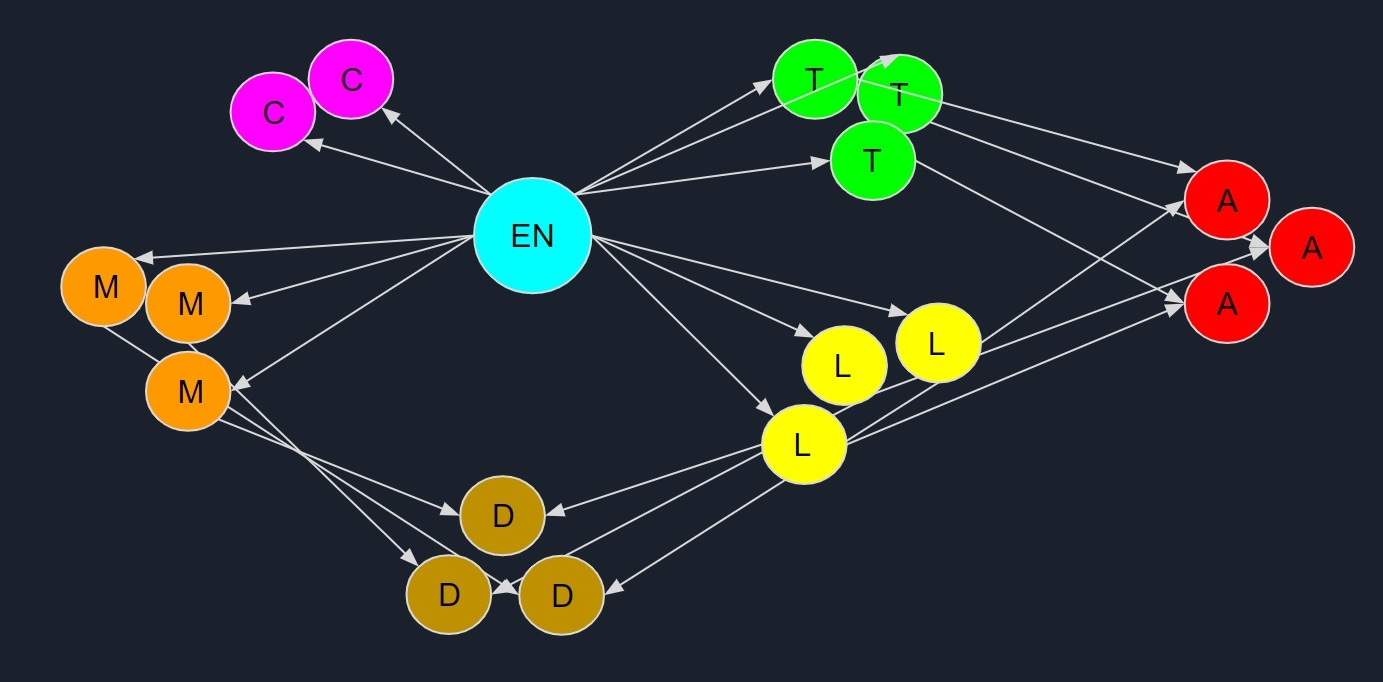
\includegraphics[width=0.5\textwidth]{04_Physical Systems Dependent & Independent Variables.jpg}
	\caption{\textit{The above structural graph represents an unfiltered R-K model, where EN stands for the central Event Node based on the choice of an arbitrary lens representing a physical phenomenon or entity. T, L, M \& C Represent the mutually-independent clusters  of Time, Length, Mass and Charge. A \& D represent the derived/dependent clusters of Acceleration and Density respectively.}}
	\label{fig:PhysicalSystems}
\end{figure}

\subsubsection{Non Physical Systems with Knowledge-Graphs}
\label{sec:NonPhysical}

The Datasets pertaining to “Non-Physical Systems” must contain a well-define Knowledge Graph related to a specific domain Ontology that contains parent nodes with 3 or more mutually independent attributes to meet the the minimum criteria of  generating an  R-K Diagram in accordance with consistent Topological Properties that can be distinguished using distinct Divergence criteria.

Such independent attributes should allow for the classification and separation of variables based on direct or derived relationships with fundamental physical dimensions and associated independent variables such as:

E.g. Age of a person can be separated as a time variable while the weight of the person is a derived from the independent mass variable and the height of that person can be separated as a length variable. All other attributes have a secondary/ derived dependence on the fundamental independent variables. However, the R-K Pipeline would allow for the addition/classification of any  additional domain specific independent variables based on a specific domain ontology relevant in a non-scientific commercial use-case such as in the case of the Tableau Super Store Dataset.\cite{TableauSuperStore}

\subsubsection{Derived Relationships}
Derived relationships are relationships that are determined by the data itself, and are learned during analysis. For example, it may be possible to derive an ontology from physical system consisting existing fudemental measures such as mass, time, and length in order to obtain derived measures such as force, momentum, and acceleration.

\subsubsection{Data Assumptions}

A directed relationship exists between metrics $M$ such the formula $Edge_{M_{i} \to M_{j}}$ would describe a directed relationship between $M_{1}$ and $M_{2}$. For the approach to be effective, there exists some combinations of filter and linkage functions, such that optimized they can segregate topological structures.

Furthermore, it is assumed that there exists a method to compare two variables (i.e over distances). Practically, this means all data needs to have some numeric based encoding to be compared.

\subsubsection{Limitations}
Such as described by the Section 4.2 in Data Criteria, this imposes the following limitations on data fed into the pipeline:

Low dimensional data, with less than 3 independent dimensions will not be compliant with the data criteria and are not suitable for this approach. Three mutually independent dimensional attributes are required to make simplicial complexes and add structure ot the data and so lacking rank would impact the structure. Additionally, data with unclear relationships between measures may be less effective than data with clear relationships between measures because a lot of the power of the R-K Models come from a hierarchical embedding, which if unclear, limits the ability for the models to perform as they should.

As an example, in the Iris dataset \cite{iris_dataset}, all measures are built off the fundamental quantity: length. In spite have 4 columns (sepal width, sepal length, petal width, petal length), all columns are inter-dependent and are not mutually independent and therefore cannot be clustered into separate independent attributes of the central iris event node, other than length, thereby resulting in non-unique Topological signatures and the failure to generate  R-K Diagrams.

\subsubsection{Ontology}

In the figure below, we describe a dendrogram with a specific ontology. An ontology in the context of an R-K Model, describes the relationship between two or more measures in the form of a hierarchy. Ontological frameworks have numerous advantages, such that it makes domain assumptions on data explicit and/or to share a common understanding of structural information across metrics. \cite{ben_mahria_chaker_zahi_2021}. The ontologies can either be learned such as with the Mahria et. al paper titled \textit{A novel approach for learning ontology from relational database: from the construction to the evaluation} or formulaized by domain experts \cite{ben_mahria_chaker_zahi_2021}. There are numerous ontological databases available for describing relationships between known domains. The Web Ontology Language (OWL) is a specific set of web standards and language devised to standardize ontologies through \textit{OWL Documents}. \cite{owl_semantic_web_standards_2012}.

In the figure below, we define a strict ontology in the store sales data. This provides the basis on which all R-K Models are formed. Any R-K Model most have some strict ontological backbone, such as the below, and compliant with data assumptions in 4.2.4 to be valid.

\begin{figure}[H]
	\centering
        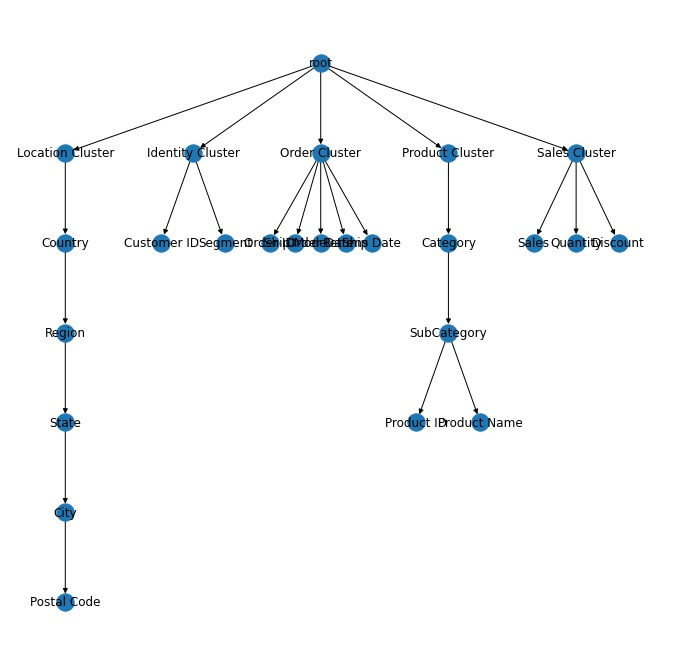
\includegraphics[width=0.5\textwidth]{images/ss_dendrogram.png}
	\caption{\textit{}}
	\label{fig:nodemask}
\end{figure}


\subsection{R-K Pipeline}

The foundational component of any R-K Diagram is an R-K Pipeline. At a base level, the R-K Pipeline can be understood as a Directed Acyclic Graph (DAG) as defined in section 2.3.1, which provides transformational components that result in an composite model we call an R-K Model. Transforms in an R-K Pipeline can be chained against each other, as long as egress from one component complies with the ingress specifications from another component. We can mathematically represent this with the following representation: $\lbrace C_{0}, C_{1}, C_{2}..., C_{n} \rbrace \in RK_{i} $ where $C_{i}$ represents a pipeline component and the egress of $C_{i}$ is compliant with a set of constraints imposed by $C_{i+1}$'s ingress.
\begin{figure}[H]
	\centering
        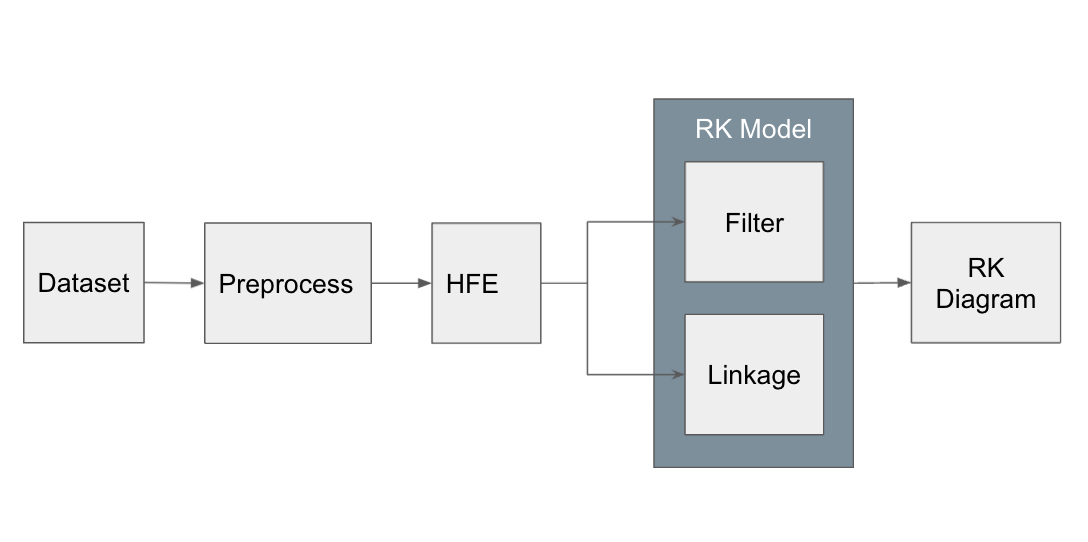
\includegraphics[width=0.5\textwidth]{images/simpliest_pipeline.png}
	\caption{\textit{The above represents a simplest R-K Pipeline. In this pipeline, data first gets preprocessed, then moved to a Hierarchical embedding function. From the hierarchy, the standard filters and links provide an R-K model. It is then forked between a compression node and a visualization node. Thus the end result is two R-K Diagrams, one compressed version and one raw version}}
	\label{fig:example_pipeline_fig}
\end{figure}

\subsection{Hierarchical Embedding Function}
\label{sec:HEF}

As discussed in Section 4.2.6, there must exist an explicit ontology related to the measures of the dataset.  Let us describe $D$ as the input dataset to the RL Toolkit. Let us describe $m_{i}$ as a measure within the set of measures $M$ such that $m_{i} \in M$. To be compliant with this proposed framework, there must exist an ontology $O$ that describes the relationship of the measures w.r.t each-other. For example, w.r.t location data, an ontology could present that a \textbf{$m_{city}$} is a child of  \textbf{$m_{state}$} which is a child of \textbf{$m_{country}$}. In the datasets that were analysed, we often provided an ontology which merged similar measures into the same ``cluster'', for example $mass_{1}$ and $mass_{2}$ were ontologically defined as part of the $Mass$ cluster in our LIGO analysis. In the Tableau Super Store Sales Dataset, we defined a custom ontology that we used for our representations. Using the R-K toolkit, one can either use pre-defined ontologies or provide custom ontologies for their data.

An Hierarchical Embedding Function ($f_{H}$) generates a graph $G$ from a set of measures $M$ such that the resulting graph $G$, is a DAG which represents a bijective mapping between $m_{i} \longleftrightarrow G_{i}$ such that all $V_{i} \in G$ can be traced back to the original value in the dataset, where $V$ is a vertex. More succinctly, $f_{H}(M) \rightarrow G$ such that $f_{H}(G_{v_{i}}) \rightarrow m_{i}$ and $f^{-1}_{H}(G_{v_{1}}) \rightarrow m_{i}$. The advantage of this requirement is that any structural graph can be inverted back into original measures used to generate the graph.

Across the pipeline, the graph generated by $H_{f}$ is referenced as a \textit{Structural Graph} ($S$). The structural graph provides the baseline ontological structure that forms the basis for all other transformations in the pipeline.

Computationally, to maintain the bijective mapping, we maintain internally a history of steps applied during the transformation such that we can easily provide the inverse function by returning the steps in reverse.

\subsection{R-K Model}

The R-K Model is the basis for any R-K Diagram. It represents the composite object that can be used to render an R-K Diagram. In that sense, an R-K Diagram the rendering of an R-K Model, and the R-K Model underlying datastructure for that render.

All R-K Models contain the following 3 components: Structural Graph, Node Masks, and Derived Links
\begin{figure}[h]
	\centering
        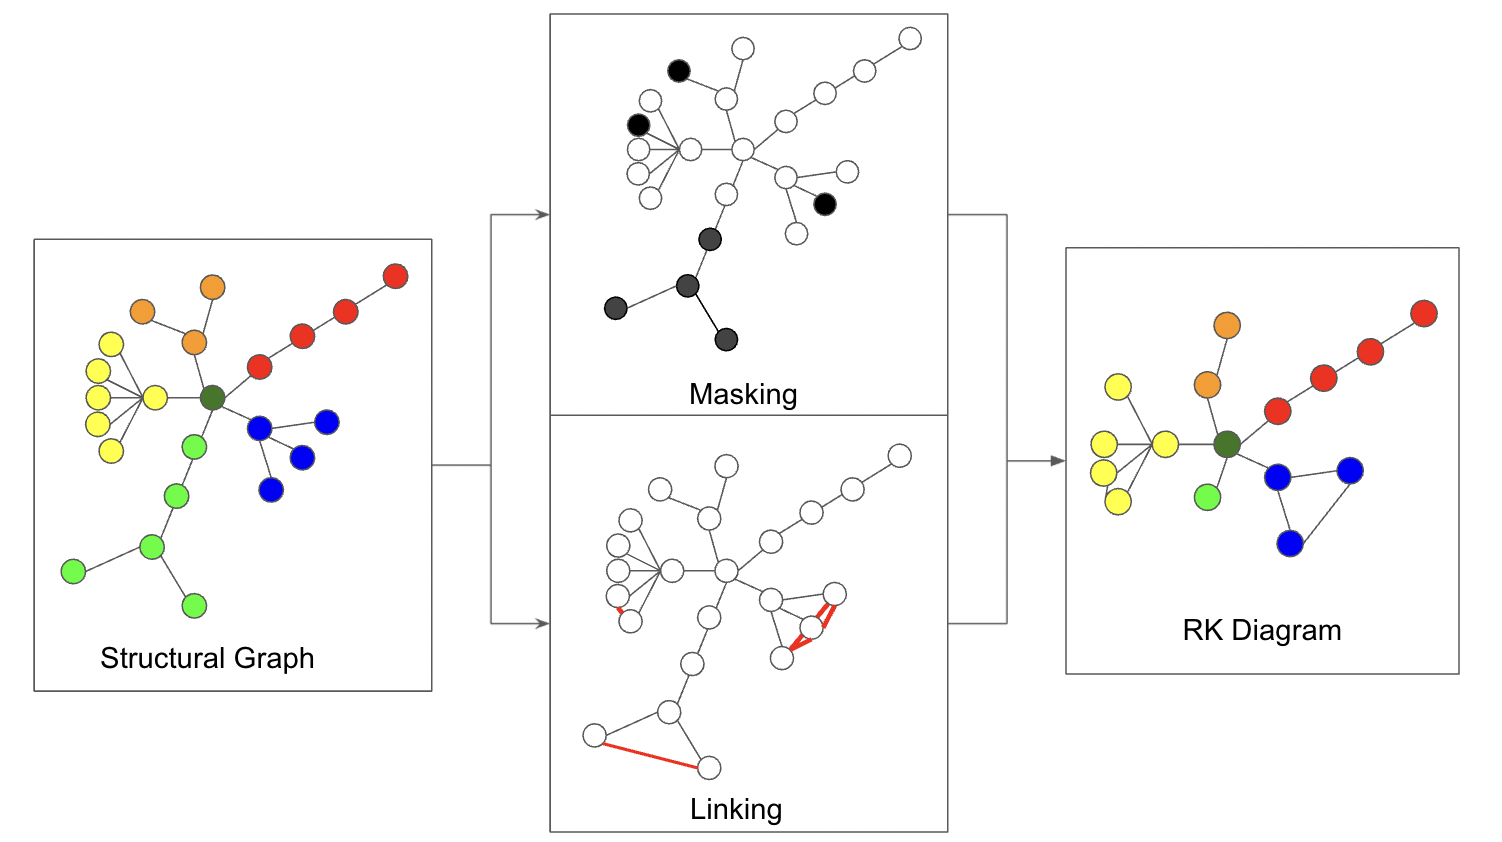
\includegraphics[width=0.5\textwidth]{images/rkmodel.png}
	\caption{\textit{The above image represents the building blocks of an R-K Model. To the left, a structural graph, which is defined in 4.7.1. In the middle, filters and linkage functions are applied resulting in the final R-K Model. The R-K Diagram is simply a rendering of the model}}
	\label{fig:fig1}
\end{figure}

Each component is described in detail below.

\subsubsection{Structural Graph}

The structural graph ($S$) is the base graph derived through the Hierarchical Embedding Function, also known as the structural graph. The structural graph provides the baseline ontological structure that forms the basis for all other transformations in the pipeline.

Because node masks are reductive operations, the number of nodes in the structural graph represents the \textit{maximal number of nodes in the R-K Diagram} such that $|nodes| \in S >= |nodes| \in R-KDiagram)$. The structural graph however does not represent that maximal number of edges. The number of possible edges in the R-K Diagram is bounded by the number of combinations of nodes in the structural graph.

The R-K Filters (described below), can bound the possible combinations of edges to less than the number in the original combinatorial graph.

In the case below, we demonstrate two forms of structural graphs. The first is the initial structural graphs that were derived off the Store Sales data outlined in the next section. The second structural graph is built off of similar data, however some nodes were expanded out. Both are viable candidates for structural graphs.

\begin{figure}[H]
	\centering
        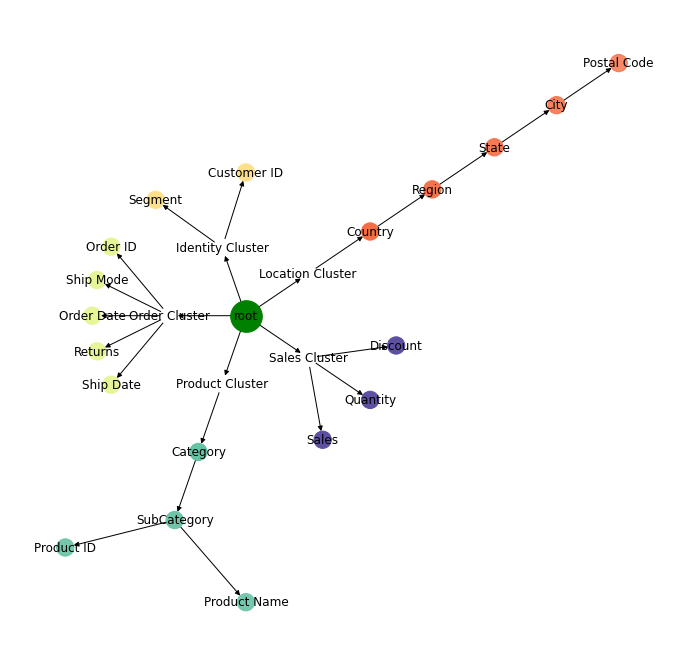
\includegraphics[width=0.5\textwidth]{images/base_hierarchy.png}
	\caption{\textit{The base structural graph of the Store Sales Data}}
	\label{fig:fig1}
\end{figure}


\begin{figure}[H]
	\centering
        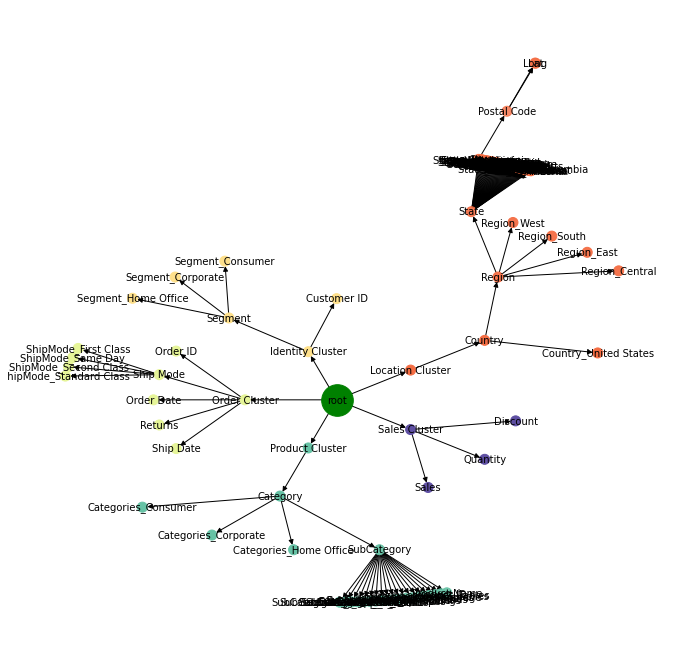
\includegraphics[width=0.5\textwidth]{images/expanded_node_structure.png}
	\caption{\textit{An expanded structural graph}}
	\label{fig:fig1}
\end{figure}

\subsubsection{Node Masks and Functions}
\label{sec:Filters}
A node mask represents a masking structure that when applied to a structural graph $S$, reduces the number of nodes into a subgraph $S^{'}$. The node masks are binary operators, which when set to \textit{true}, filter a node and it's direct children.

To derive the node masks, we produce a set of filters $F_{n}(G)$, which takes in a graph and returns a mask. We define Filter Functions  w.r.t. Simplicial Complexes formed by a combination of nodes and edges, such that filtration of a simplicial complex K is a nested family of subcomplexes $(Kr)r \in T$, where $T \subseteq R$, such that for any,r; $r \prime \in T$  if $r \le r \prime$ then $Kr \subseteq Kr\prime$,  and  $K=Ur \in TKr$. The subset T may be either finite or infinite. More generally, a filtration of a topological space M is a nested family of subspaces $(Mr)r \in T$,  where $ T  \subseteq R $, such that for anyr; $r\prime \in T$, if $r \le r\prime$ then $Mr \subseteq Mr\prime$ and, $M=Ur_{\in}TMr$. For example, if $f : M \rightarrow R$ is a function, then the family $Mr = f-1 ((-\infty , r \rbrack), r \in R$ %defines a filtration called the sublevel set filtration of f. In practical situations, the parameter $r \in T$ can often be interpreted as a scale parameter and belong to the set of filtrations classically used in TDA.

In the pipeline, one can combine multiple filter functions together. The union of the filters provide the final node mask, such that $ F_{n}(G) \cup N_{m}$, where $N_{m}$ is the node mask.

\begin{figure}[H]
	\centering
        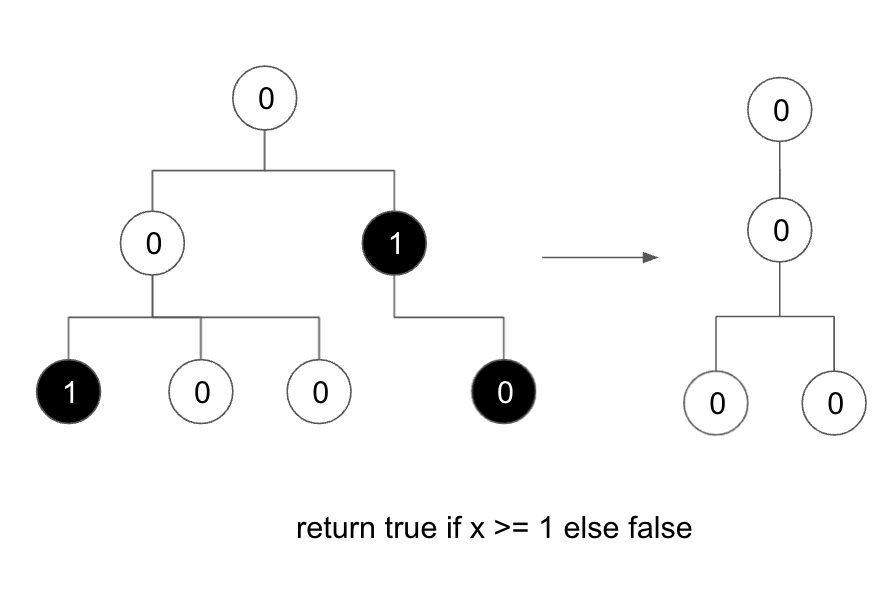
\includegraphics[width=0.5\textwidth]{images/nodemask.png}
	\caption{\textit{An example node masks with a filter of >= 1. All nodes and children of the nodes are removed that have a value >= 1 and applied at the root level. Different filters can be applied to different subgraphs.}}
	\label{fig:nodemask}
\end{figure}

\subsubsection{Linkers}

In order to define linkages we must begin with the following mathematical consideration. Let $G = (V, E)$ be an undirected graph without multiple edges or loops. Let $n =|V|$ and $e= |E|$. The linkage of G is defined to be the maximum min-degree of any of the subgraphs of G (the min-degree of a subgraph is the least degree of any of its vertices; the degree of a vertex is taken relative to the subgraph). The width of G is defined to be the minimum, over all linear orderings of the vertices of G, of the maximum, with respect to any vertex v, of the number of vertices connected with v and preceding it in the linear ordering. It has also been mathematically proven in Topology that the width of a graph is equal to its linkage.

Furthermore, according to the French Mathematician Erdös, it has been proven that every graph G has a subgraph with min-degree at least equal to the density $[e/n]$ of G. Therefore, the density is a lower bound for the linkage (equivalently, width) of graphs with given numbers of edges and vertices. Given a positive integer j, if in the definition of width we consider not the number of vertices preceding and connected with v but rather the least number of vertices preceding and connected with any cluster of at most j consecutive vertices extending to the right up to v, we get a graph parameter known as j-width.

\begin{figure}[H]
	\centering
        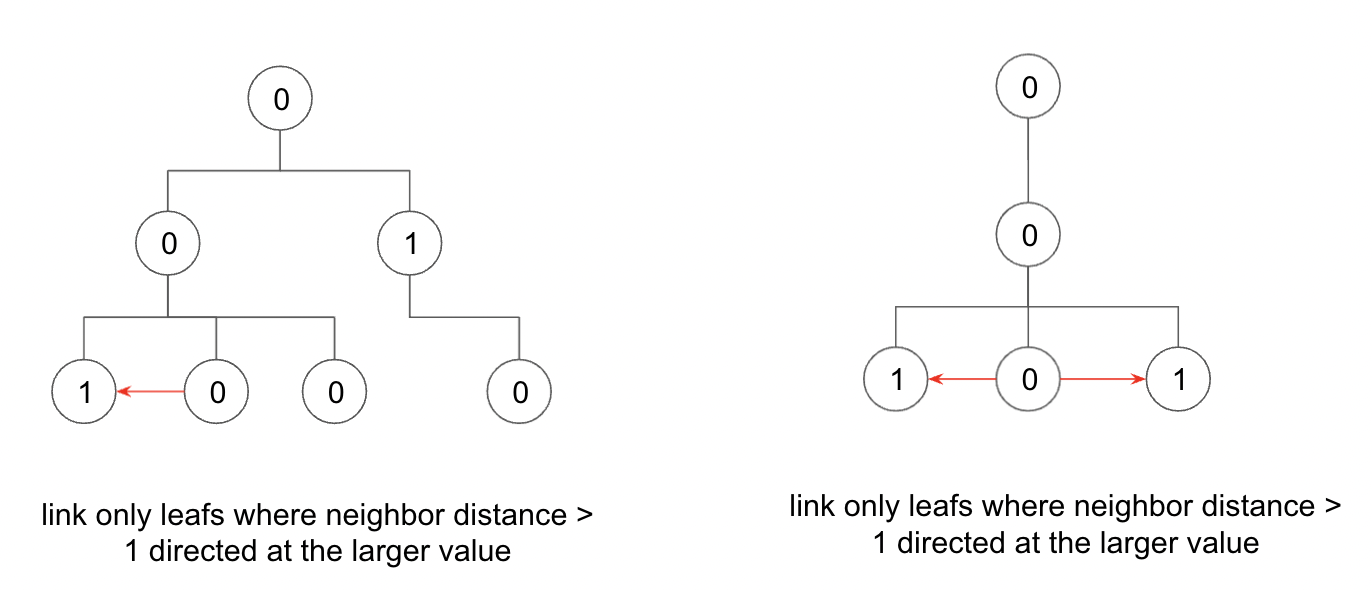
\includegraphics[width=0.5\textwidth]{images/linkage.png}
	\caption{\textit{Example of a linker function. The same linker function are applied to two different graphs, providing directed edges across leafs.}}
	\label{fig:linker}
\end{figure}

\subsubsection{Linkage Math}

Let be a layout of a graph $G (V, E)$, i.e., a linear ordering $v_{1} ,..., v_{n}$ of its vertices. The width with respect to of a set S ${v_{i}^{-k+1},...,v_{i}}$ of k consecutive vertices (notationally widthl(S)) is defined to be the number of vertices $\lbrace v_1,...,v_{i-k} \rbrace$ in the set adjacent to vertices in S $(1 \le i \le k \le n)$. Informally, the width of S with respect to is the number of vertices preceding S and adjacent to elements of S.

Informally, the width of S with respect to is the number of vertices preceding S and adjacent to elements of S.Now, let j be an integer such that $1 \le j \le n$. The j-width of a vertex v with respect to is the least width of any set of at most min (i,j) consecutive vertices extending to the right up to vi, i.e.,

$j-widthl(vi) = min \lbrace widthl(vi-k+1,...,vi):k =1,..., min(i,j)\rbrace$

The j-width of G with respect to l is defined to be the maximum of j-widthl(vi) over all vertices v of G.

The j-min-degree of a subgraph H of G is the minimum ext-degreeH(S) over all sets S of vertices of H with $1 \le |S| \le j$. Obviously, the 1-min-degree of a subgraph is the least degree of its vertices.The j-linkage of G is the maximum j-min-degree of any subgraph of G. Obviously, the l-linkage of G is the maximum min-degree of any of its subgraphs. The l-linkage of G is simply called the linkage of G.Furthermore, it has been proven mathematically that for any graph $G(V, E)$,, the j-width of G is equal to its j-linkage.

\subsubsection{Choice of Lens}
\label{sec:sectionlens}

The choice of lens is critical for the basis of ontology and the R-K Model. Is is the lens at which an ``event'' is determined from, such that ``Lens'' defines the root node such that all branching nodes and the hierarchy are birthed from the choice of lens. As an example, in the store sales data, there may exist many lenses, such as a Customer lens, or a Transaction lens. Each lens would provide unique events associated with such events, with different structural graphs as the foundation for each R-K Diagram.

\begin{figure}[H]
	\centering
        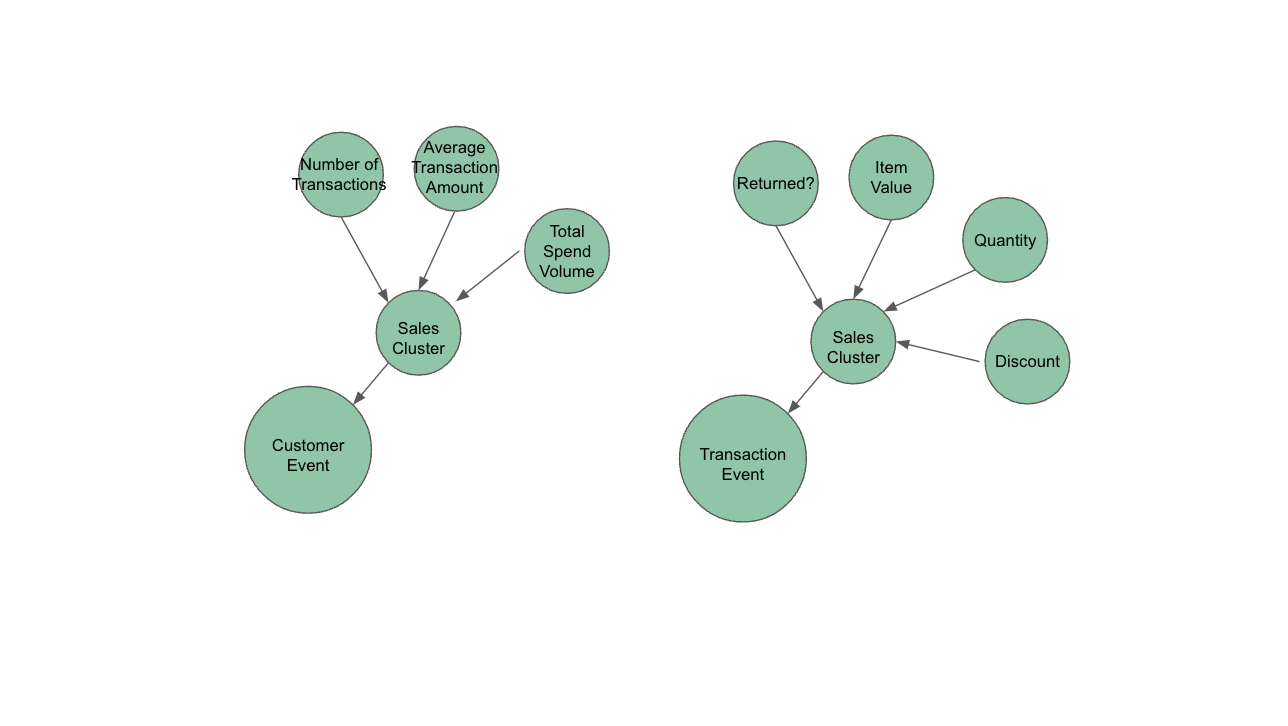
\includegraphics[width=0.5\textwidth]{images/lens_choice.png}
	\caption{\textit{The diagrams above show the effect of the lens on the structural graph. To the left, a lens is chosen from a specific ``Customer'' event. To the right, a lens is chosen from a ``transactions'' perspective. The values and metrics associated with each lens are related to the respective lens. }}
	\label{fig:linker}
\end{figure}

\subsubsection{R-K Diagram}

An RK-Diagram is the render of an RK-Model. Given an RK-Model, an R-K Diagram renders the R-K Model in 2 or 3d space. As an R-K Model is multi-dimensional representation of data, an R-K diagram can display many dimensions in 2D, without data loss that a typical projection model would have.

We tend to use a radial layout for our demonstrations, but any graph layout can be used, with a preference toward deterministic layouts. We prefer deterministic layouts, because it allows easier qualitative comparisons of R-K Diagrams and their differences.

\begin{figure}[H]
	\centering
        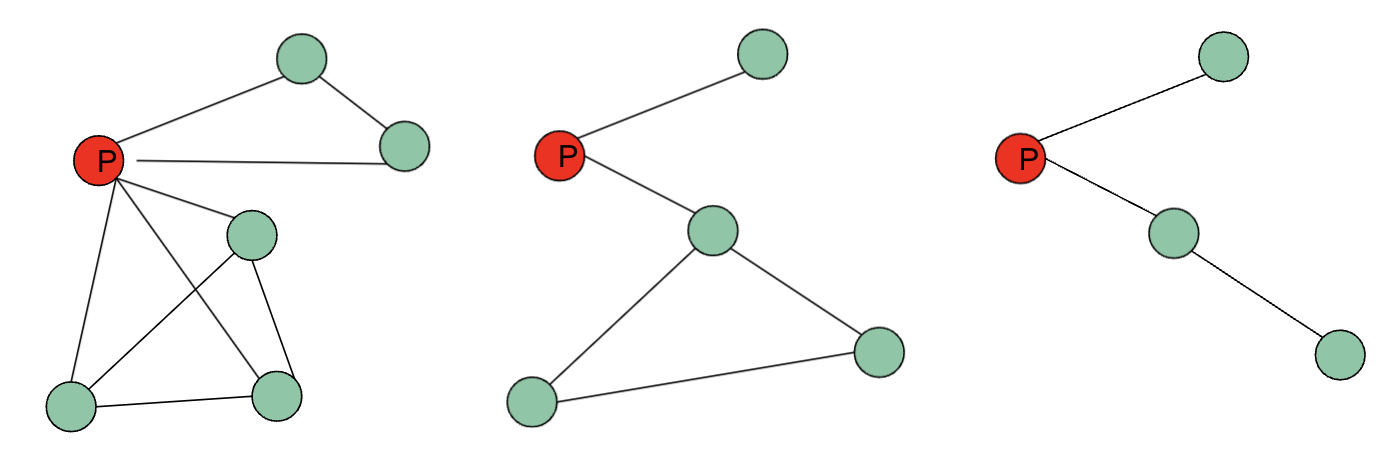
\includegraphics[width=0.5\textwidth]{images/rk-diagram-layouts.png}
	\caption{\textit{In the R-K Diagrams above, we use a deterministic layout which makes it easier to spot the differences between R-K Diagrams based on visual features}}
	\label{fig:linker}
\end{figure}

\subsubsection{Betti Number Analysis for Macroscopic Topological Classification}
\label{sec:BettiNumber}
In this paper, we have only explored topological similarity and divergence measures that are calculated with respect to a combined study of nodes, directed edges, properties of DAGs and corresponding Topological distance measures between any 2 R-K diagrams. However, the R-K pipeline and R-K models are built in a way to allow for the smooth establishment of homotopy equivalence between any 2 well defined spaces unlike point cloud data where such equivalence is not established by default. Hence, this allows for effective ways to compute the number of independent j-dimensional surfaces for higher dimensional embeddings on R-K diagrams in Phase-Space. 

This would in tern also allow for smooth ways to drive and obtain the $j-th$ Betti Numbers which would lead to a formalised method to count the number of loops present in unique event-based topological signatures. Thus new metrics can be established to compute and classify the global macroscopic properties of R-K diagrams, thereby leading to the quantification of additional parameters for machine learning templates which bring about further enhancements to the R-K pipeline for the classification and segregation of different R-K diagrams with more distinct divergence measures.
 
\subsection{Measuring R-K Distance}
\label{sec:rk_distance}

Critical to the tuning and understanding of R-K Diagrams is the ability to quantitatively measure distance (and in the dual, similarity) across R-K Diagrams. There is a plethora of existing research that has been done on understanding topological and graph distances in Phase Space. For example, in Hilaga et. al, they analyzed a Reeb graph, and using TDA, computed the geodesic normalized distance, where the geodesic distance of a surface from the formula $\mu(v) = \int_{p \in S} g(v,p)dS$ where $g(v,p)$ returns geodesic distance of points u and v on a mesh. \cite{hilaga_shinagawa_kohmura_kunii}. This approach was not well suited for our analysis, because we do not create a mesh in an R-K Diagram, however demonstrates one of many potential ways to compare topological structures against eachother.

Another approach by Máté et. al use multiple approaches in \textit{A topological similarity measure for proteins}, in which they use a geometric approach using the Jaccard distance and Hausdorff distance based on the barcodes used in persistent homology. \cite{máté_hofmann_wenzel_heermann_2014}. Various other appropriate metrics exist that we will not cover in this section but refer to in the citations. \cite{mazandu_mulder_2012} \cite{reuter_2009}

In our implementation, we used a weighted distance function $d(G_{1}, G_{2})\times{w}$ by applying composite distance function based on geometric and value distance, where the geometric distance was implemented over a Jaccard distance based upon nodes and edges, and the value distance was computed using the Mahalanobis distance similar to Salleh et. al\cite{Salleh1_et_al}. The final distance equation can be supplied through the following:

\begin{equation}
D(G_{i},G_{j}) = f(T,V)\times{w}
\end{equation}

where $f(T,V)$ is a composite function based on topological distance $T$ and value distance $V$ weighted by vector $w$.

Our approach was inspired by Máté et. al's geometric measures and after concieving of such a method, later found Salleh et. al's using Mahalanobis distance with Jaccard's distance in the paper that validated a simliar approach in \textit{Combining Mahalanobis and Jaccard Distance to Overcome Similarity Measurement Constriction on Geometrical Shapes} \cite{Salleh1_et_al}, in which they combined Mahalanobis and Jaccard distance in a weighted average to provide similarity measures across metrics.

\subsubsection{Topological Distance}
\label{subsec:topological_distance}

As mentioned in \hyperref[sec:rk_distance]{Measuring R-K Distance} section, we used Jaccard distance to provide the geometric distance across R-K Diagrams. The Jaccard distance is one of many possible distance functions that can be applied toward graph distances. It is simple but effective in many machine learning algorithms and is a widely applied algorithm across many domains. \cite{roughgarden_valiant_2021}. The formula can be described as:

\begin{equation}
J(A,B) = \frac{| A \bigcap B |}{| A \bigcup B |}
\end{equation}

where A and B are a tuple that represents an edge $V_{i} \to V_{j}$ that $V_{i}$ is the source node and $V_{j}$ is the sink.

To be appropriate for the R-K Diagrams, it is critical to evaluate the Jaccard distances against the \textit{directed edges}, such that the distance measure is sensitive to topological differences due to direction. If a Jaccard distance is applied only at the vertex level, key information about the directed edges and the linked vertexes would be lost. This would be ineffective in the R-K Diagram approach hence we utilized Edges for Jaccard measurements, such that critical features in the distance measurement are preserved.

\subsubsection{Value Distance}
\label{subsec:valuedistance}

The value distance is intended to amplify the effects of the distance measure when topology isn't sufficient to demonstrate differences. For example, in the case of store sales, a purchase could be very similar topologically, but very different in terms of magnitude as the actual sales value differ radically across R-K Diagrams. By comparing the magnitude of the nodes as well as the topology, it provides a clear distinction when topological differences are not sufficient.

There are various methods to compute the value distance that can be effective. Salleh et. al use the Mahalanobis distance as a method to measure the ``Value Distance'' of a graph.  We applied the Mahalanobis distance to provide the distance mesaure. Mahalanobis can be computed by the formula: \cite{Salleh1_et_al}

\begin{equation}
d_{MH}(G_{1}, G_{2}) = \sqrt{(\bar{x}-\bar{y})^{T}\Sigma^{-1}(\bar{x}-\bar{y})}
\end{equation}

where: $\bar{x}$ and $\bar{y}$  are the means of the data, $(\bar{x}-\bar{y})^{T}$ is the transposed of the differences of the mean and $\sum^{-1}$ is the inverse covariance matrix.

We compute the Mahalanobis distance across the entire dataset, and then normalize the values to between 0 and 1 such that we are bound between $[0,1]$ pre-weighting.

\begin{figure*}[t]
	\centering
        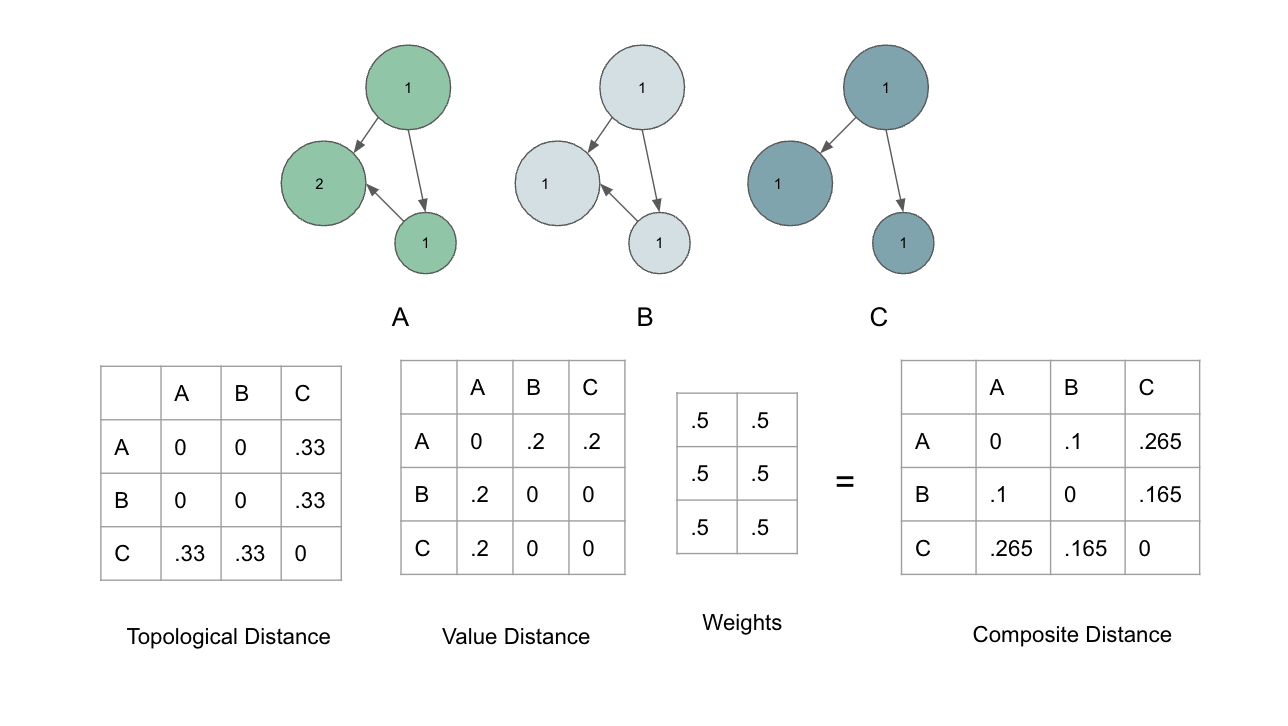
\includegraphics[width=1\textwidth]{images/value_cost.png}
	\caption{\textit{In the top row, all three diagrams have the same topologies but very different values. The value function, encodes this as an important piece of information when comparing the distance of the diagrams between each-other. On the bottom, the bottom left is more topologically similar to the middle such that the cost topologically to the center is 0 where the cost of the bottom right would be greater than 0 because there is a missing edge. }}
	\label{fig:sample store sales dataset}
\end{figure*}

\subsubsection{Combining the values into a composite distance score}
\label{subsec:distance_score_composite}

We finally combine the Value Distance and the Topological Distance into a composite distance score by the function:

\begin{equation}
D(G_{i},G_{j}) = f(T,V)\times{w}
\end{equation}

where $T$ and $V$ are bound by the range $[0,1]$ and $\sum{w} = 1$. This provides us a final distance score in the range $[0,1]$. This can be expressed by the following:

\begin{equation}
D(G_{i}, G_{j}) = \frac{\sum_{i=1}^{n}x_{i}w_{i}}{\sum_{i=1}^{n}w_{i}}
\end{equation} \cite{Salleh1_et_al}

Where
\begin{equation}
\sum_{i=0}^{n}{w_{i}} = 1
\end{equation}
\subsubsection{Similarity}
\label{subsec:similarity}

As our results are normalized between 0 and 1, we can compute the similarity as the dual of the distance, such that $Sim(G_{i}, G_{j}) = 1-D(G_{i}, G_{j}) = 1-f(T,V)\times{w}$.

\subsection{Future work on distances}
\label{subsec:future_distance_work}
We acknowledge that there is still much research that can be done to improve our distance models and provide more robust measures for R-K Diagram comparisons. The proposal in the above sections outline a starting point for future research.

\subsubsection{Homotopy \& Persistent Homology of R-K Diagrams}
The  Hierarchical Embedding Function ($f_{H}$) of R-K diagrams always ensures that it generates a graph $G$ from a set of measures $M$ such that the resulting graph $G$, is a DAG which represents a bijective mapping between $m_{i} \longleftrightarrow G_{i}$ such that all $V_{i} \in G$ can be traced back to the original value in the dataset. This is also consistent with respect to ontological relationships between dependent and independent variables which form the basic simplex clusters of our fundamental structural graphs - $G$. The advantage of this requirement is that any structural graph can be inverted back into original measures used to generate the graph. Now, since the structural graph provides the baseline ontological structure that forms the basis for all other transformations in the R-K pipeline.

Hence, it ensures that all R-K models consistently render R-K diagrams that are Homotopic with respect to their topological properties and would allow for the smooth computation of persistence diagrams between topologically similar R-K diagrams such as the topological signatures of  BH-BH mergers or NS-NS merger signals from LIGO data. These signatures would preserve the same global topological properties of invariance and persistence under continuous deformations of shape, due to the well defined nature of simplicial complexes consisting of interconnected DAGs which eventually give rise to the fundamental structural graphs of all R-K diagrams.Thus it could be quantified both mathematically and computationally and explored as a part of future research on the study of Homotopy \&  Persistent Homology of different R-K Diagrams.

\subsubsection{Isometric Compressions, Inverse Function, and Decompression}

With R-K Diagrams, we employ isometrically compressible techniques which maintain state change history to provide compression and decompression functions. The compression techniques must be lossless. We can define a compression function $C(G)$, that given a graph returns a compressed version of the graph $G\prime$ where the number of nodes and edges is equal to or less than $G$. We restrict compressible techniques to require an inverse function, such that $G\prime + \nabla{G} = G$. This is critical for the ability to transition between levels of compression.

Because an R-K Diagram can represents a projection that can display many dimensions in 2D space, compression of the R-K Diagram also isometrically projects the diagram into a lower dimensional space, however the visualization can still be visualized at the same space.

Graph compression models have been well evaluated in academia. For example, Gelbert et. al, \cite{gilbert_levchenko} explore various compression techniques focused on semantic compression, based on: degree, a parameter Beta (which weighs neighbourhood of a cluster), paths, an algorithm called KeepOne and KeepAll, and redundant vertex elimination. \cite{gilbert_levchenko}

In the first version of the R-K Toolkit, we have shown a limited implementation of graph compression via a 1 degree leaf compressible technique, which compresses all 1 degree leafs into a single leaf branching from the parent node. The steps are maintained internally so that the $G$ can be reconstructed from $G\prime$. We intend to extend the compressible techniques to others, including those implemented in the Gilbert et al. paper, but did not in the interest of executing the first completed version of the pipeline.

\begin{figure}[H]
	\centering
        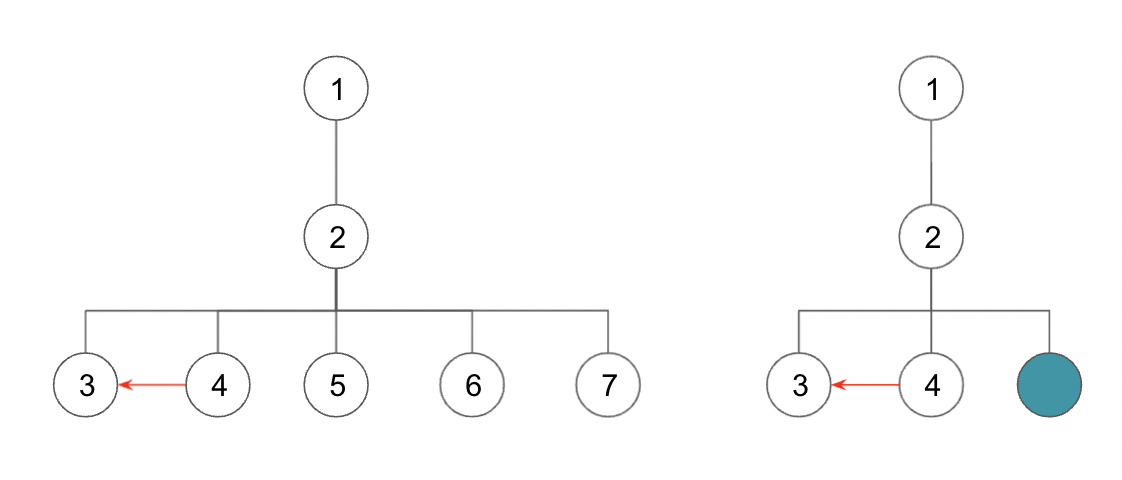
\includegraphics[width=0.5\textwidth]{images/compression_example2.png}
	\caption{\textit{We employed a simple compression model. In this example, nodes 5,6, and 7 are compressed into a single node.}}
	\label{fig:linker}
\end{figure}


\subsection{R-K Extensibility and Flexibility}

The R-K Toolkit and concepts explored in the implementation are a general framework and way of thinking about the data, not a specific implementation. However, each component is intended to be implemented in a way that can be optimized for a particular domain and use case.
